\documentclass[a4paper, 14pt]{extarticle}

% Поля
%----------------------
\usepackage{geometry}
\usepackage{tikz}
\usepackage{svg}
\usepackage{float}
\usetikzlibrary{arrows.meta, automata, positioning}
\geometry{a4paper,left=2cm,right=1cm,
    top=2cm,bottom=2cm,bindingoffset=0cm}
%----------------------

% Russian-specific packages
%----------------------
\usepackage[T2A]{fontenc}
\usepackage[utf8]{inputenc}
\usepackage[english, main=russian]{babel}
%----------------------

\usepackage{textcomp}

% Красная строка
%----------------------
\usepackage{indentfirst}
%----------------------

% Graphics
%----------------------
\usepackage{graphicx}
\usepackage{mathtools}
\graphicspath{ {./images} }
\usepackage{wrapfig}
%----------------------

% Import minted
%----------------------
\usepackage{minted}
%----------------------

% Href
%----------------------
\usepackage{hyperref}
\usepackage{xcolor}
 % Цвета для гиперссылок
\definecolor{linkcolor}{HTML}{799B03} % цвет ссылок
\definecolor{urlcolor}{HTML}{799B03} % цвет гиперссылок
\hypersetup{pdfstartview=FitH,  linkcolor=linkcolor,urlcolor=urlcolor, colorlinks=true}
%----------------------

\linespread{1.3}
\sloppy
\clubpenalty=10000
\widowpenalty=10000

\begin{document}

%--------------------------------------
%			ТИТУЛЬНЫЙ ЛИСТ
%--------------------------------------
\begin{titlepage}
\thispagestyle{empty}
\newpage


%Шапка титульного листа
%--------------------------------------
\vspace*{-60pt}
\hspace{-65pt}
\begin{minipage}{0.3\textwidth}
\hspace*{-20pt}\centering

\includegraphics[width=\textwidth]{emblem}
\end{minipage}
\begin{minipage}{0.67\textwidth}\small \textbf{
\vspace*{-0.7ex}
\hspace*{-6pt}\centerline{Министерство науки и высшего образования Российской Федерации}
\vspace*{-0.7ex}
\centerline{Федеральное государственное бюджетное образовательное учреждение }
\vspace*{-0.7ex}
\centerline{высшего образования}
\vspace*{-0.7ex}
\centerline{<<Московский государственный технический университет}
\vspace*{-0.7ex}
\centerline{имени Н.Э. Баумана}
\vspace*{-0.7ex}
\centerline{(национальный исследовательский университет)>>}
\vspace*{-0.7ex}
\centerline{(МГТУ им. Н.Э. Баумана)}}
\end{minipage}
%--------------------------------------

%Полосы
%--------------------------------------
\vspace{-25pt}
\hspace{-35pt}\rule{\textwidth}{2.3pt}

\vspace*{-20.3pt}
\hspace{-35pt}\rule{\textwidth}{0.4pt}
%--------------------------------------

\vspace{1.5ex}
\hspace{-35pt} \noindent \small ФАКУЛЬТЕТ\hspace{80pt} <<Информатика и системы управления>>

\vspace*{-16pt}
\hspace{47pt}\rule{0.83\textwidth}{0.4pt}

\vspace{0.5ex}
\hspace{-35pt} \noindent \small КАФЕДРА\hspace{50pt} <<Теоретическая информатика и компьютерные технологии>>

\vspace*{-16pt}
\hspace{30pt}\rule{0.866\textwidth}{0.4pt}
  
\vspace{11em}

\begin{center}
\Large {\bf Лабораторная работа № 4} \\ 
\large {\bf Вариант 16} \\
\large {\bf по курсу <<Теория формальных языков>>} \\
\end{center}\normalsize

\vspace{8em}


\begin{flushright}
  {Студент группы ИУ9-52Б Прадхан М. Р. \hspace*{15pt}\\ 
  \vspace{2ex}
  Преподаватель Непейвода А.Н. \hspace*{15pt}}
\end{flushright}


\bigskip

\vfill
 

\begin{center}
\textsl{Москва} \\
\textsl{15 января 2026}
\end{center}
\end{titlepage}
%--------------------------------------
%		КОНЕЦ ТИТУЛЬНОГО ЛИСТА
%--------------------------------------

\newpage

\section{Задание}
Дано расширенное регулярное выражение: 
\[
\hat{ } \Big( \big( (?: a | b)^* \big) \backslash 2 \backslash 2 \, a \, \big( (?: a | b)^* \big) \, b \, \backslash 3 \Big) \backslash 1? \$
\]
Имеющуюся регулярку:
\begin{itemize}
\item[---] Проанализировать на КС-свойство, в случае его наличия — на регулярность.
\item[---] Построить "наивный"парсер слов для языка, используя рекурсивный разбор
с возвратами. Парсер не должен зацикливаться.
\item[---]  Построить оптимизированный парсер слов для языка. Оценить сверху его
вычислительную сложность.
\item[---]  Посредством фазз-тестирования проверить эквивалентность парсеров и построить сравнительные графики скорости их работы на случайных словах,
принадлежащих языку, и не принадлежащих языку (два тестовых пула).
\end{itemize}
\newpage

\section{КС-свойство}
Дано выражение:
\[
\hat{ } \Big( \big( (?: a | b)^* \big) \backslash 2 \backslash 2 \, a \, \big( (?: a | b)^* \big) \, b \, \backslash 3 \Big) \backslash 1? \$
\]

Тогда обозначим:
\[
x \in \{a,b\}^* \text{ — то, что захватывает } ((?:a|b)^*) \text{ (группа 2)}
\]

\[
y \in \{a,b\}^* \text{ — то, что захватывает } ((?:a|b)^*) \text{ (группа 3)}
\]

Тогда внутренняя группа (группа 1) задаёт строку:
\[
x\, x\, x\, a\, y\, b\, y
\]

А всё выражение задаёт язык:
\[
L = \{ (x x x a y b y)^k \mid x,y \in \{a,b\}^*, \, k \in \{1,2\} \}
\]

Пересечём язык $L$ с регулярным языком 
\[
R = a^* a^* a^* a b a^*
\]

Тогда получаем:
\[
L \cap R = \{ a^n a^n a^n a a^m b a^m \mid n,m \ge 0 \}
\]

Представим $L \cap R$ как объединение двух подъязыков, где $n=m$ и $n \neq m$.  
Возьмём:
\[
L' = \{ a^n a^n a^n a a^n b a^n \mid n \ge 0 \}
\]

С помощью леммы о накачке для контекстно-свободных языков докажем, что $L'$, а значит и исходный язык, не является КС.  

Пусть наше слово:
\[
w = a^p a^p a^p a a^p b a^p
\]

Разобьём $w$ на части $uvxyz$ так, чтобы выполнялись условия леммы о накачке:
\[
|vxy| \le p, \quad |vy| \ge 1, \quad uv^kxy^kz \in L \text{ для всех } k \ge 0
\]

Рассмотрим все варианты накачки:
\begin{enumerate}
    \item Накачивая отдельно блок из $a^p$, мы выходим из структуры языка.
    \item Накачивая отдельно или в промежутке $a$ или $b$, мы опять выходим из структуры языка.
    \item Накачивая соседние блоки, состоящие из $a^p$, вне зависимости от синхронности, мы также выходим из языка.
\end{enumerate}

Следовательно, $L'$ не контекстно-свободен, а значит и исходный язык $L$ не является контекстно-свободным.

\section{Наивный парсер}

Наивный парсер следующим образом проверяет принадлежность слова языку, соответствующему регулярному выражению 
\[
\hat{ } \Big( \big( (?: a | b)^* \big) \backslash 2 \backslash 2 \, a \, \big( (?: a | b)^* \big) \, b \, \backslash 3 \Big) \backslash 1? \$
\]

\begin{enumerate}
    \item Перебираются все возможные длины префикса $X$ слова.
    \item Для каждого $X$ проверяется условие обратной ссылки: оставшаяся часть слова либо пустая, либо равна $X$.
    \item Внутри $X$ перебираются все возможные длины $Y$, чтобы проверить, что префикс $X$ имеет вид $YYY a Z b Z$, где $Z$ — произвольная подстрока.
    \item Если найдена комбинация $Y$ и $Z$, полностью удовлетворяющая структуре $X$, слово принимается; иначе — отклоняется.
\end{enumerate}

\section{Оптимизированный парсер}

Оптимизированный парсер следующим образом проверяет принадлежность слова языку с регулярным выражением
\[
\hat{ } \Big( \big( (?: a | b)^* \big) \backslash 2 \backslash 2 \, a \, \big( (?: a | b)^* \big) \, b \, \backslash 3 \Big) \backslash 1? \$
\]

\begin{enumerate}
    \item Перебираются все возможные длины $Y$, префикса подстроки $X$, который должен соответствовать $YYY a Z b Z$.
    \item Для каждого $Y$ проверяется, что первые $3Y$ символа повторяют $Y$ трижды (т.е. $YYY$).
    \item Проверяется наличие символа \texttt{a} после $YYY$.
    \item Перебираются все допустимые длины $Z$, и проверяется, что $Z b Z$ полностью совпадает с соответствующими символами строки.
    \item Вычисляется длина $X$ как $3|Y| + 1 + 2|Z| + 1$. Проверяется остаток строки: если он пуст или равен $X$ (для обратной ссылки \texttt{\textbackslash 1?}), слово принимается.
\end{enumerate}

В отличие от наивного парсера, этот метод не перебирает все возможные $X$ и минимизирует количество создаваемых строк \texttt{slice}, что ускоряет проверку на длинных словах.

\subsection*{Оценка вычислительной сложности}

Обозначим $n$ — длину слова.  
\begin{itemize}
    \item Перебор $Y$ выполняется максимум $O(n)$ раз ($yLen \le n/3$).
    \item Для каждого $Y$ перебирается $Z$ с длиной до $O(n)$.
    \item Внутри каждого $Z$ выполняется проверка $Z b Z$ и остатка X, которая требует максимум $O(n)$ операций посимвольно.
\end{itemize}

Таким образом, верхняя оценка сложности алгоритма:
\[
O(n) \text{ (по } Y) \times O(n) \text{ (по } Z) \times O(n) \text{ (проверка X/остатка) } = O(n^3)
\]

На практике реальная скорость гораздо выше из-за раннего выхода при несоответствиях и ограничений на длину $Z$, что сильно сокращает количество итераций.

\section{Графики скорости работы парсеров}

\begin{figure}[h]
\centering
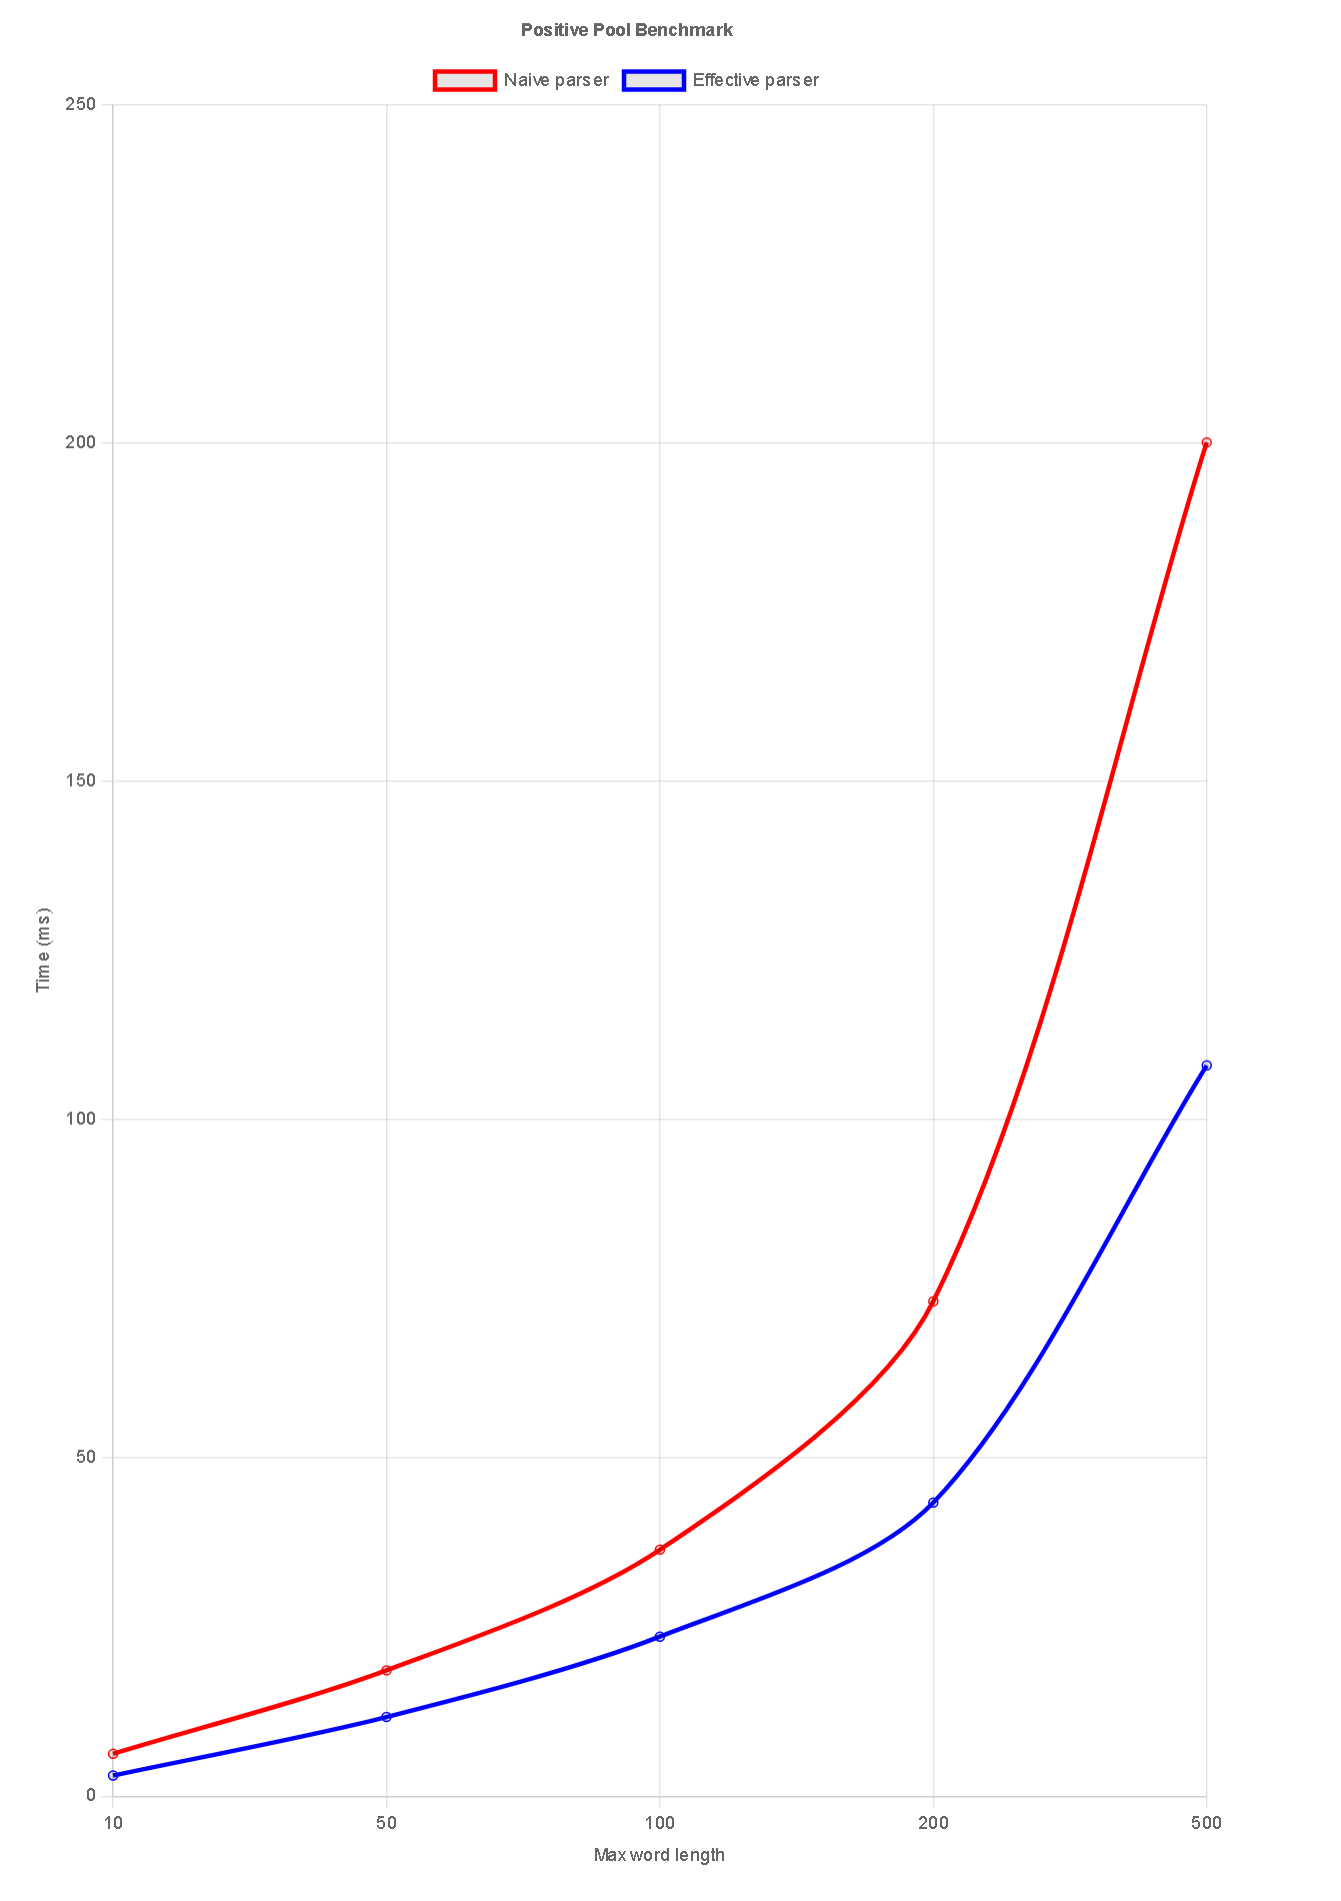
\includegraphics[width=0.6\textwidth]{img/positive_pull.PNG}
\caption{График времени работы парсеров на пулле слов, принадлежащих языку}
\end{figure}

\begin{figure}[h]
\centering
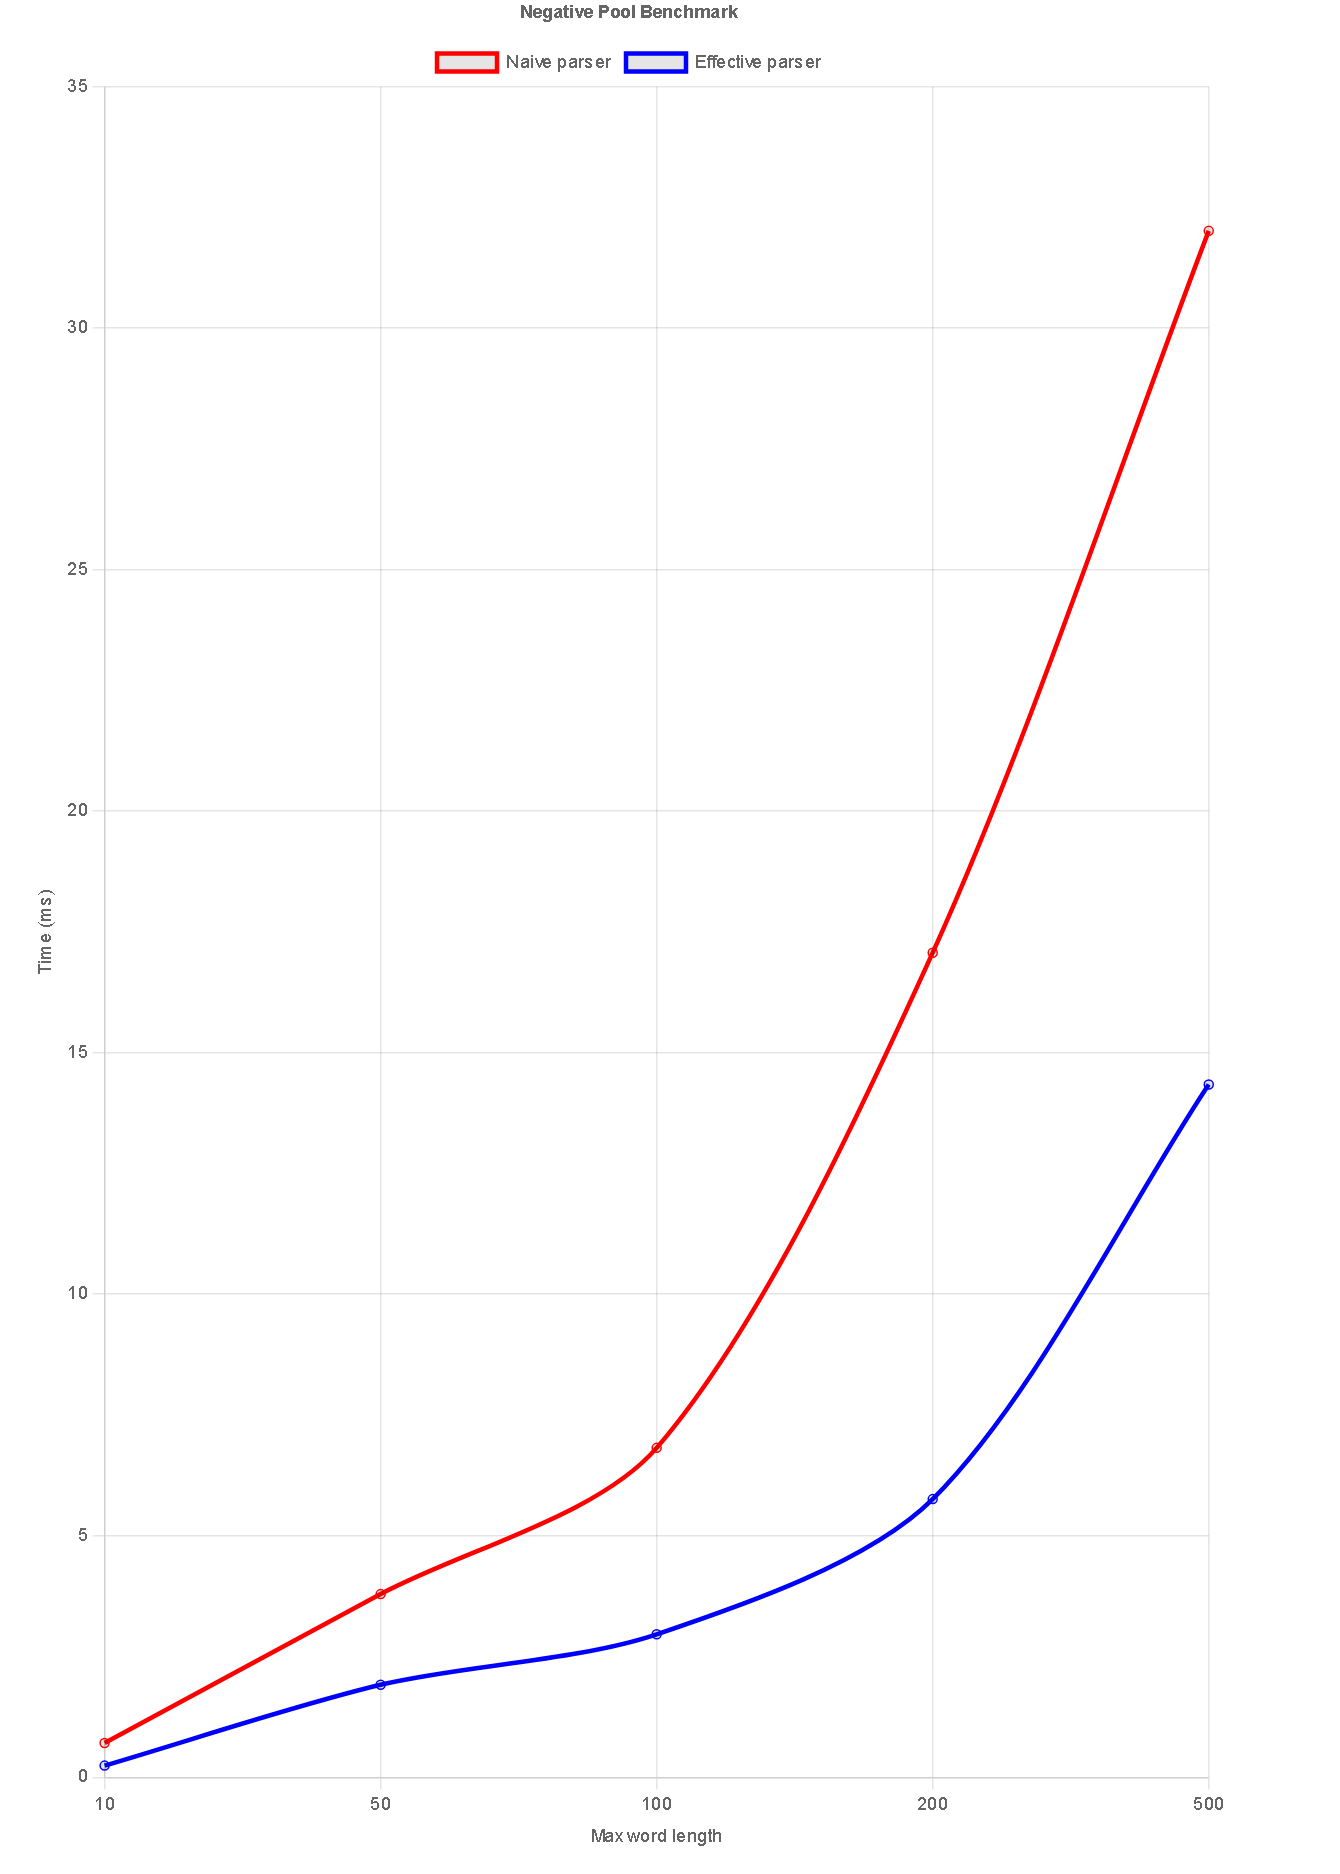
\includegraphics[width=0.6\textwidth]{img/negative_pull.PNG}
\caption{График времени работы парсеров на пулле слов, не принадлежащих языку}
\end{figure}


\end{document}


